%Przykładowy plik ułatwiający złożenie projektu dyplomowego inżynierskiego.
%UWAGA: Generowany napis na stronie tytułowej o treści PROJEKT DYPLOMOWY INŻYNIERSKI został zaproponowany przeze mnie i nie jest, póki co, potwierdzony przez władze wydziału. Przed ostatecznym oddaniem tak złożonej pracy należy upewnić się jaka powinna być treść tego napisu. W momencie gdy uzyskam informację na temat treści tego napisu, dokonam niezbędnych zmian w źródłach.

\documentclass[eng,printmode]{mgr}
%opcje klasy dokumentu mgr.cls zostały opisane w dołączonej instrukcji

%poniżej deklaracje użycia pakietów, usunąć to co jest niepotrzebne
\usepackage{polski} %przydatne podczas składania dokumentów w j. polskim
%\usepackage[polish]{babel}%alternatywnie do pakietu polski, wybrać jeden z nich
\usepackage[utf8]{inputenc} %kodowanie znakĂłw, zaleĹĽne od systemu
\usepackage[T1]{fontenc} %poprawne składanie polskich czcionek

%pakiety do grafiki
\usepackage{graphicx}
\usepackage{subfigure}
\usepackage{psfrag}

%pakiety dodające dużo dodatkowych poleceń matematycznych
\usepackage{amsmath}
\usepackage{amsfonts}

%pakiety wspomagające i poprawiające składanie tabel
\usepackage{supertabular}
\usepackage{array}
\usepackage{tabularx}
\usepackage{hhline}

%pakiet wypisujący na marginesie etykiety równań i rysunków zdefiniowanych przez \label{}, chcąc wygenerować finalną wersję dokumentu wystarczy usunąć poniższą linię
\usepackage{showlabels}

%definicje własnych poleceń
\newcommand{\R}{I\!\!R} %symbol liczb rzeczywistych, działa tylko w trybie matematycznym
\newtheorem{theorem}{Twierdzenie}[section] %nowe otoczenie do składania twierdzeń

%dane do złożenia strony tytułowej
\title{Aplikacja do identyfikacji i rozpoznawania twarzy użytkownika w celu zabezpieczenia dostępu przy użyciu technologii Qt}
\engtitle{Qt based secure access application using face detection and identification}
\author{Dominik Guderski}
\supervisor{dr inż. Andrzej Rusiecki, W-4/K-9}
%\guardian{dr hab. inż. Imię Nazwisko Prof. PWr, I-6} %nie używać jeśli opiekun jest tą samą osobą co prowadzący pracę
\graphicspath{ {../img/}}
%\date{2008} %standardowo u dołu strony tytułowej umieszczany jest bieżący rok, to polecenie pozwala wstawić dowolny rok

%poniżej jest lista kierunków i specjalności na wydziale elektroniki, należy wybrać właściwe lub dopisać jeśli nie ma odpowiednich
\field{Automatyka i Robotyka (AIR)}
\specialisation{Technologie Informacyjne w Systemach Automatyki (ART)}
%\specialisation{Robotyka (ARR)}
%\specialisation{Komputerowe sieci sterowania (ARK)}
%\specialisation{Systemy informatyczne w automatyce (ASI)}
%\specialisation{Komputerowe systemy zarzÄ…dzania \\procesami produkcyjnymi (ARS)}
%\field{Elektronika i telekomunikacja (EIT)}
%\specialisation{Akustyka (ETA)}
%\specialisation{Aparatura elektroniczna (EAE)}
%\specialisation{Elektroniczne i komputerowe \\systemy automatyki (ESA)}
%\specialisation{Zastosowania inĹĽynierii komputerowej \\w technice (EZI)}
%\specialisation{Inżynieria dźwięku (EID)}
%\specialisation{Elektronika stosowana \\i optokomunikacja (TEO)}
%\specialisation{Telekomunikacyjne sieci szerokopasmowe (TSS)}
%\specialisation{Teleinformatyczne sieci mobilne (TSM)}
%\specialisation{Sygnały w telekomunikacji cyfrowej (TSC)}
%\specialisation{Teleinformatyczne systemy rozsiewcze (TSR)}
%\field{Informatyka (INF)}
%\specialisation{Systemy informatyki w medycynie \\i technice (IMT)}
%\specialisation{InĹĽynieria systemĂłw informatycznych (INS)}
%\specialisation{InĹĽynieria internetowa (INT)}
%\specialisation{Systemy i sieci komputerowe (ISK)}
%\field{Teleinformatyka (TIN)}
%\specialisation{Teleinformatyka (TIN)}

%tutaj zaczyna się właściwa treść dokumentu
\begin{document}
\bibliographystyle{plabbrv} %tylko gdy uĹĽywamy BibTeXa, ustawia polski styl bibliografii

\maketitle %polecenie generujące stronę tytułową
\dedication{6cm}{Projekt dedykuję rodzicom.}

\tableofcontents %spis treści

%poniżej znajduje się przykładowa treść dalszej części dokumentu, zainteresowanych zachęcam do rozszyfrowania frazy "Lorem ipsum" :)

\chapter{Wstęp}

Rozpoznawanie twarzy jako technika biometryczna służąca do identyfikacji osób wykształciła się jako obiekt zainteresowań naukowców w latach osiemdziesiątych XX wieku. Pierwsze komercyjne systemy powstały w latach dziewięćdziesiątych XX wieku.\cite{historyreco}

Główną cechą rozpoznawania twarzy jest bezinwazyjność. Wystarczy spojrzenie w obiektyw. Systemy wykrywające i rozpoznające twarz wymagają szczególnych warunków otoczenia do poprawnego działania. Zmiany oświetlenia, położenia twarzy względem urządzenia rejestrującego mogą w znaczny sposób zaburzyć działanie algorytmu detekcji i rozpoznawania twarzy. W skrajnych przypadkach zmiana oświetlenia lub zmiana położenia twarzy względem urządzenia rejestrującego może uniemożliwić działanie algorytmów.
\section{Cel i zakres programu}
Niniejsza praca dotyczy praktycznego zagadnienia zabezpieczania dostępu do zasobów. Autor zaimplementował dwuelementowe uwierzytelnianie. Sprawdzana jest znajomość zdefiniowanego wcześniej hasła dla danego użytkownika oraz porównywana jest twarz odczytana z kamery z informacjami zawartymi w bazie danych. Moduł uwierzytelniania i obsługi informacji o użytkownikach został zaimplementowany przez autora od podstaw. Za bazę do stworzenia algorytmu identyfikacji oraz rozpoznawania twarzy posłużyła biblioteka openCV. Głównym celem było stworzenie programu, który realizowałbym zadanie kontrolowania dostępu do zasobów poprzez rozpoznawanie twarzy w czasie rzeczywistym porównując z twarzami wzorcowymi oraz sprawdzanie znajomości hasła.

\section{Koncepcja rozwiązania problemu}
By zrealizować idee uwierzytelniania użytkownika na podstawie hasła oraz zdjęcia twarzy potrzebne są dwa elementy. Baza danych zawierająca nazwę użytkownika i hasło, oraz baza danych zawierająca wzorcowe zdjęcia twarzy powiązane z użytkownikiem. Oczywiście kwestią implementacyjną jest czy owe bazy będą jednym obiektem, czy też dwoma. W wypadku opisywanego projektu wybrane zostało podejście dwóch baz. Oczywiście obie te bazy są ze sobą synchronizowane i razem tworzą koncepcyjnie jedną bazę danych, nazywaną dalej bazą danych użytkowników.
\subsection{Przechowanie nazwy użytkownika i hasła}
Uwierzytelnianie użytkowników wymaga bazy danych. Owa baza została zrealizowana przy pomocy dwóch elementów. Pierwszy z nich to plik .face\_recognizerrc, który przechowuje nazwę użytkownika oraz zakodowane hasło, w zdefiniowanym przez program formacie(zdefiniowanym w taki sposób by ułatwić przetwarzanie pliku przez program). Format ten ma postać:\\
::nazwa\_użytkownika::zakodowane\_hasło::\\
::nazwa\_użytkownika2::zakodowane\_hasło2::
\\
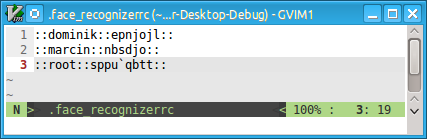
\includegraphics{face}


Czyli dla każdego użytkownika przeznaczona jest jedna linia w pliku. Nazwa użytkownika jest umieszczona w sposób niezakodowany, natomiast hasło umieszczone jest w sposób zakodowany prostym szyfrem Cezara. Celem autora nie była implementacja nietrywialnego algorytmu szyfrowania hasła, ponieważ przyjęte zostało założenie, iż pliki konfiguracyjne programu są umieszczone w bezpiecznej lokalizacji. Można to osiągnąć uruchamiając program z konta administratora(wtedy pliki konfiguracyjne mogą zostać umieszczone w katalogu chronionym przed odczytem przez innych użytkowników niż administrator).
\\

Innym rozwiązaniem jest uruchomienie programu w dowolnym miejscu, jednak ograniczenie interface'u poprzez który użytkownicy programu mogą sterować programem. Takim ograniczeniem może być odpowiednie przygotowanie systemu operacyjnego, tak by uruchomiony program zajmował całą dostępna przestrzeń ekranu. Dodatkowo użytkownik ma do dyspozycji ekran dotykowy by móc sterować działaniem programu. Nie ma możliwości przełączenia czy też włączenia innego procesu w systemie. Takie podejście może zostać zastosowane przy projektowaniu interface'u do sterowania inteligentnym budynkiem lub pomieszczeniem.

\subsection{Przechowywanie wzorcowych zdjęć twarzy}
Program oprócz wspomnianego pliku przechowującego dane tekstowe tworzy także katalog .face\_recognizer. W tym katalogu dla każdego użytkownika z wyjątkiem użytkownika root(administrator) istnieje katalog o nazwie odpowiadającej nazwie użytkownika.
\\
.face\_recognizer/\\
\textbullet nazwa\_użytkownika/\\
\textbullet nazwa\_użytkownika2/\\

Katalog ten w momencie dodania użytkownika do bazy danych jest wypełniany dostarczonymi przez użytkownika  pięcioma wzorcowymi zdjęciami twarzy. Wzorce te w momencie próby uzyskania dostępu do systemu przez użytkownika są porównywane z obrazem wykrytej twarzy z kamery podłączonej do systemu.

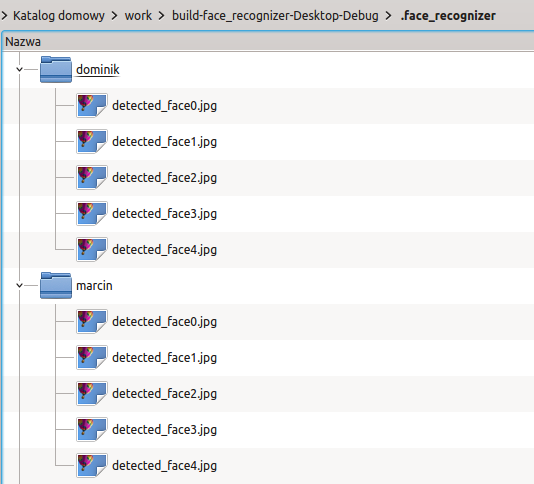
\includegraphics{dir}
\subsection{Konto administratora}
Wyjątkowym przypadkiem, o którym należy wspomnieć jest konto administratora(login: root, domyślne hasło: root\_pass). Owe konto jako jedyne jest dostępne już przy pierwszym uruchomieniu programu z domyślnym hasłem dostarczonym razem z programem. Bardzo ważna ze względów bezpieczeństwa jest zmiana domyślnego hasła. Wymaganiem stawianym administratorowi podczas procedury uwierzytelniania jest podanie prawidłowego hasła. Nie jest sprawdzany obraz z kamery. Oprócz tego konto root nie posiada katalogu root w katalogu .face\_recognizer/, gdyż nie jest on potrzebny. Konto administratora jest potrzebne by dodawać i usuwać użytkowników.

\subsection{Detekcja i rozpoznawanie twarzy}
W celu detekcji i rozpoznawania twarzy została użyta biblioteka OpenCV. Detekcja twarzy odbywa się przy użyciu funkcji Haar-like, umożliwiającej dość dobrą i szybką detekcję obiektów. Rozpoznawanie jest zrealizowane za pomocą metody EigenFace.

Podstawowy problem- szybkość przetwarzania obrazu, który zależy od mocy obliczeniowej komputera oraz zaimplementowanego algorytmu. Ważna kwestią jest poprawność wykrywania twarzy. W wypadku gdy algorytm wykryje twarz w miejscu gdzię rzeczywiście jej nie ma może to prowadzić do błędnego działania programu, a także oznacza marnowanie zasobów. Z tego powodu w programie został przyjęty minimalny rozmiar wykrytej twarzy (50x50 pixeli). Wykryte obiekty mniejsze od tej granicznej wielkości nie są przetwarzane.

\section{Układ pracy}
We wstępie został opisany temat pracy, poruszone w niej zagadnienia oraz problemy związane z tematyką. W rozdziale drugim przedstawiono opis zagadnień teoretycznych związanych z tematem pracy. Opisano metody oraz biblioteki użyte w procesie realizacji założen projektu. W podsumowaniu znajdują się wnioski czego udało się dokonać, czego udało się uniknąc i co sprawiło problemy. Podana też została propozycja jednej ze ścieżek dalszego rozwoju aplikacji.
\chapter{Podstawy teoretyczne}
Quisque nibh sapien, lobortis posuere, dignissim id, ultricies ut, est. Cras nec nunc nec ligula placerat ullamcorper. Maecenas consequat consequat nisi.


\section{Przetwarzanie obrazów}
Nulla quis enim ut erat rutrum feugiat. Suspendisse lacinia tempor mi. Vestibulum nec lacus sed est rutrum cursus. Cras ultrices est eget ped
\section{Rozpoznawanie twarzy}
Aliquam quis sem. Phasellus tincidunt fringilla metus. Sed id purus.

\section{Uwierzytelnianie użytkownika}
Proin venenatis nisl eget erat. Cum sociis natoque penatibus et magnis dis parturient montes, nascetur ridiculus mus
\begin{itemize}
\item Mauris nonummy lorem at orci.
\item Donec accumsan aliquam libero.
\item Donec fringilla ultricies diam.
\item Nulla venenatis est non ligula.
\item Morbi in mi convallis dolor accumsan egestas.
\item Sed euismod nibh in nulla.
\item Sed rhoncus lorem at lectus.
\item Pellentesque fermentum rutrum dui.
\end{itemize}

Proin euismod. Curabitur adipiscing ipsum ac augue. Maecenas hendrerit tortor non velit suscipit laoreet. Aenean tempus. Nunc c

\chapter{Opis programu}
\section{Użyte algorytmy}
Nulla a nisl at nisl dignissim facilisis. In sit amet mi. Nunc ullamcorper, ligula vel aliquam pretium, nulla mauris euismod ipsum, sit amet tempus massa nulla non elit. Donec congue. Nulla purus. Aenean dui orci, ornare quis, interdum sed, molestie ac, tellus. Lorem ipsum dolor sit amet, consectetuer adipiscing elit. Quisque mollis diam nec elit. Maecenas nec enim. Maecenas facilisis urna quis arcu. Fusce posuere.

\section{Użyte technologie}
Nam laoreet sagittis massa. Cum sociis natoque penatibus et magnis dis parturient montes, nascetur ridiculus mus. Morbi nulla. Cras eu dolor. Praesent et purus. Praesent mi turpis, ullamcorper ut, adipiscing eget, dictum ut, felis. Phasellus a metus. Etiam vulputate gravida pede. Aenean sit amet massa quis libero dapibus mattis. Suspendisse potenti. Cras placerat.
citudin ligula.

\section{Struktura programu}
Maecenas augue justo, iaculis ut, laoreet ac, ullamcorper sed, velit. In sollicitudin. Phasellus cursus nisl vitae urna auctor fermentum. Integer purus ipsum, tristique non, consectetuer pharetra, convallis ac, metus. Vestibulum nec nulla. Fusce convallis, dui nec dignissim dignissim, pede ipsum iaculis est, quis rhoncus nulla lorem nec nibh. Quisque viverra. Phasellus ac quam ac orci mattis dapibus. Sed id neque. Praesent at elit in enim vestibulum ornare. Aenean mauris enim, auctor nec, lacinia ut, pulvinar sit amet, diam.

\section{Interface użytkownika}
Proin nisl velit, blandit vitae, rhoncus et, ullamcorper nec, turpis. Quisque placerat sagittis odio. Ut non arcu. Morbi fringilla scelerisque erat. Duis mattis nulla vitae nisi consectetuer vehicula. Ut ultricies hendrerit velit. Vestibulum dignissim. Pellentesque feugiat, enim quis vehicula porttitor, eros quam blandit libero, sed ultrices lacus enim in urna. Vestibulum vitaus.

 non, sagittis vel, faucibus sed, lacus. Sed consectetuer, velit nec aliquam imperdiet, ipsum nunc vehicula urna, non ultricies odio odio eget dui. Donec venenatis erat a diam. Phasellus vel neque.

\chapter{Wyniki eksperymentów}

Etiam scelerisque vulputate nulla. Phasellus facilisis vehicula lectus. Nullam adipiscing nisi sit amet sapien. Cras tristique. Cum sociis natoque penatibus et magnis dis parturient montes, nascetur ridiculus mus. Cras laoreet urna sit amet est. Nunc faucibus. Integer bibendum ipsum a nunc. In non nisl. In elit elit, consequat et, nonummy vel, sollicitudin sed, felis. Mauris elit libero, malesuada non, sagittis vel, faucibus sed, lacus. Sed consectetuer, velit nec aliquam imperdiet, ipsum nunc vehicula urna, non ultricies odio odio eget dui. Donec venenatis erat a diam. Phasellus vel neque.

\chapter{Podsumowanie}
Etiam scelerisque vulputate nulla. Phasellus facilisis vehicula lectus. Nullam adipiscing nisi sit amet sapien. Cras tristique. Cum sociis natoque penatibus et magnis dis parturient montes, nascetur ridiculus mus. Cras laoreet urna sit amet est. Nunc faucibus. Integer bibendum ipsum a nunc. In non nisl. In elit elit, consequat et, nonummy vel, sollicitudin sed, felis. Mauris elit libero, malesuada non, sagittis vel, faucibus sed, lacus. Sed consectetuer, velit nec aliquam imperdiet, ipsum nunc vehicula urna, non ultricies odio odio eget dui. Donec venenatis erat a diam. Phasellus vel neque.

\appendix
\chapter{Doxygen}

Sed augue orci, porttitor vitae, rhoncus id, molestie nec, sem. Maecenas non nisi a risus porta dapibus. Curabitur ut mi. Morbi a est sed lacus rutrum ornare. Duis tempus luctus tellus. In hac habitasse platea dictumst. Nullam purus dui, consequat consequat, dignissim et, molestie sit amet, neque. Phasellus orci arcu, semper eget, mollis vel, imperdiet sed, mi. Nulla erat enim, ornare id, pellentesque id, placerat ac, ipsum. Proin vestibulum rhoncus pede. Praesent placerat pharetra arcu. Aenean interdum ipsum rutrum nisl. Curabitur lacinia tincidunt sapien. Nunc sem mauris, molestie in, egestas ac, porta at, erat.
.

Vestibulum eget nulla non est eleifend ultricies. Nam cursus nisi ac ante. Quisque sagittis dictum dui. Nullam faucibus molestie augue. Nulla facilisi. Sed ut magna. Fusce facilisis sodales libero. Nulla nonummy lacus quis leo. Aenean a libero. In pretium ornare diam. Mauris sed eros ut mauris tempor fringilla. Donec nunc pede, pretium fringilla, gravida eu, laoreet ut, pede.
\addcontentsline{toc}{chapter}{Bibliografia} %utworzenie w spisie treści pozycji Bibliografia
%\bibliography{bibliografia} % wstawia bibliografię korzystając z pliku bibliografia.bib - dotyczy BibTeXa, jeżeli nie korzystamy z BibTeXa należy użyć otoczenia thebibliography
\begin{thebibliography}{12}

\bibitem{masteringopencv} Daniel Lelis Baggio, Mastering OpenCV with Practical Computer Vision Projects
\bibitem{learningopencv} Adrian Kaehler, Gary Bradski, Learning OpenCV 2nd Edition
\bibitem{guiqt} Jasmin Blanchette, Mark Summerfield, C++ GUI Programming with Qt 4, Second Edition
\bibitem{boost} http://www.boost.org/doc/
\bibitem{stl} http://www.cplusplus.com/reference/
\bibitem{opencv} http://docs.opencv.org/
\bibitem{cleancode} Robert C. Martin, Czysty kod. Podręcznik dobrego programisty
\bibitem{facedetection} http://www.multimedia-computing.de/mediawiki//images/5/52/MRL-TR-May02-revised-Dec02.pdf
\bibitem{historyreco} History of Face Recognition http://vismod.media.mit.edu/tech-reports/TR-516/node7.html
\end{thebibliography}

%opcjonalnie może się tu pojawić spis rysunków i tabel
% \listoffigures
% \listoftables
\end{document}

